\documentclass[a4paper, 14pt]{extarticle}

% Поля
%--------------------------------------
\usepackage{geometry}
\geometry{a4paper,tmargin=2cm,bmargin=2cm,lmargin=3cm,rmargin=1cm}
%--------------------------------------


%Russian-specific packages
%--------------------------------------
\usepackage[T2A]{fontenc}
\usepackage[utf8]{inputenc} 
\usepackage[english, main=russian]{babel}
%--------------------------------------

\usepackage{textcomp}

% Красная строка
%--------------------------------------
\usepackage{indentfirst}               
%--------------------------------------             


%Graphics
%--------------------------------------
\usepackage{graphicx}
\graphicspath{ {./images/} }
\usepackage{wrapfig}
%--------------------------------------

% Полуторный интервал
%--------------------------------------
\linespread{1.3}                    
%--------------------------------------

%Выравнивание и переносы
%--------------------------------------
% Избавляемся от переполнений
\sloppy
% Запрещаем разрыв страницы после первой строки абзаца
\clubpenalty=10000
% Запрещаем разрыв страницы после последней строки абзаца
\widowpenalty=10000
%--------------------------------------

%Списки
\usepackage{enumitem}

%Подписи
\usepackage{caption} 

%Гиперссылки
\usepackage{hyperref}

\hypersetup {
	unicode=true
}

%Рисунки
%--------------------------------------
\DeclareCaptionLabelSeparator*{emdash}{~--- }
\captionsetup[figure]{labelsep=emdash,font=onehalfspacing,position=bottom}
%--------------------------------------

\usepackage{tempora}

%Листинги
%--------------------------------------
\usepackage{listings}
\lstset{
  basicstyle=\ttfamily\footnotesize, 
  %basicstyle=\footnotesize\AnkaCoder,        % the size of the fonts that are used for the code
  breakatwhitespace=false,         % sets if automatic breaks shoulbd only happen at whitespace
  breaklines=true,                 % sets automatic line breaking
  captionpos=t,                    % sets the caption-position to bottom
  inputencoding=utf8,
  frame=single,                    % adds a frame around the code
  keepspaces=true,                 % keeps spaces in text, useful for keeping indentation of code (possibly needs columns=flexible)
  keywordstyle=\bf,       % keyword style
  numbers=left,                    % where to put the line-numbers; possible values are (none, left, right)
  numbersep=5pt,                   % how far the line-numbers are from the code
  xleftmargin=25pt,
  xrightmargin=25pt,
  showspaces=false,                % show spaces everywhere adding particular underscores; it overrides 'showstringspaces'
  showstringspaces=false,          % underline spaces within strings only
  showtabs=false,                  % show tabs within strings adding particular underscores
  stepnumber=1,                    % the step between two line-numbers. If it's 1, each line will be numbered
  tabsize=2,                       % sets default tabsize to 8 spaces
  title=\lstname                   % show the filename of files included with \lstinputlisting; also try caption instead of title
}
%--------------------------------------

%%% Математические пакеты %%%
%--------------------------------------
\usepackage{amsthm,amsfonts,amsmath,amssymb,amscd}  % Математические дополнения от AMS
\usepackage{mathtools}                              % Добавляет окружение multlined
\usepackage[perpage]{footmisc}
%--------------------------------------

%--------------------------------------
%			НАЧАЛО ДОКУМЕНТА
%--------------------------------------

\begin{document}

%--------------------------------------
%			ТИТУЛЬНЫЙ ЛИСТ
%--------------------------------------
\begin{titlepage}
\thispagestyle{empty}
\newpage


%Шапка титульного листа
%--------------------------------------
\vspace*{-60pt}
\hspace{-65pt}
\begin{minipage}{0.3\textwidth}
\hspace*{-20pt}\centering

\includegraphics[width=\textwidth]{emblem}
\end{minipage}
\begin{minipage}{0.67\textwidth}\small \textbf{
\vspace*{-0.7ex}
\hspace*{-6pt}\centerline{Министерство науки и высшего образования Российской Федерации}
\vspace*{-0.7ex}
\centerline{Федеральное государственное бюджетное образовательное учреждение }
\vspace*{-0.7ex}
\centerline{высшего образования}
\vspace*{-0.7ex}
\centerline{<<Московский государственный технический университет}
\vspace*{-0.7ex}
\centerline{имени Н.Э. Баумана}
\vspace*{-0.7ex}
\centerline{(национальный исследовательский университет)>>}
\vspace*{-0.7ex}
\centerline{(МГТУ им. Н.Э. Баумана)}}
\end{minipage}
%--------------------------------------

%Полосы
%--------------------------------------
\vspace{-25pt}
\hspace{-35pt}\rule{\textwidth}{2.3pt}

\vspace*{-20.3pt}
\hspace{-35pt}\rule{\textwidth}{0.4pt}
%--------------------------------------

\vspace{1.5ex}
\hspace{-35pt} \noindent \small ФАКУЛЬТЕТ\hspace{80pt} <<Информатика и системы управления>>

\vspace*{-16pt}
\hspace{47pt}\rule{0.83\textwidth}{0.4pt}

\vspace{0.5ex}
\hspace{-35pt} \noindent \small КАФЕДРА\hspace{50pt} <<Теоретическая информатика и компьютерные технологии>>

\vspace*{-16pt}
\hspace{30pt}\rule{0.866\textwidth}{0.4pt}
  
\vspace{11em}

\begin{center}
\Large {\bf Лабораторная работа № 3} \\
\large {\bf по курсу <<Теория искусственных нейронных сетей>>} \\
\large <<Методы многомерного поиска. Генетический алгоритм>>
\end{center}\normalsize

\vspace{8em}


\begin{flushright}
  {Студентка группы ИУ9-72Б Самохвалова П. С. \hspace*{15pt}\\
  \vspace{2ex}
  Преподаватель Каганов Ю. Т.\hspace*{15pt}}
\end{flushright}

\bigskip

\vfill
 

\begin{center}
\textsl{Москва 2023}
\end{center}
\end{titlepage}
%--------------------------------------
%		КОНЕЦ ТИТУЛЬНОГО ЛИСТА
%--------------------------------------

\renewcommand{\ttdefault}{pcr}

\setlength{\tabcolsep}{3pt}
\newpage
\setcounter{page}{2}

\section{Цель работы}\label{Sect::goal}

\begin{enumerate}
    \item Изучение алгоритмов многомерного поиска 1-го и 2-го порядка.
    \item Разработка программ реализации алгоритмов многомерного поиска 1-го и 2-го порядка.
    \item Вычисление экстремумов функции.
    \item Изучение методов решения задач многоэкстремальной оптимизации на основе генетического алгоритма.
    \item Разработка программы реализации генетического алгоритма.
    \item Решение задачи многоэкстремальной оптимизации для заданных многоэкстремальных функций.
\end{enumerate}

\section{Задание}\label{Sect::task}

Требуется найти минимум тестовой функции Розенброка:

$f(x) = \sum_{i = 1}^{n - 1}[a(x_{i}^2 - x_{i + 1})^2 + b(x_i - 1)^2] + f_0$

\begin{enumerate}
    \item Методами сопряженных градиентов (методом Флетчера-Ривза и методом Полака-Рибьера).
    \item Квазиньютоновским методом (Девидона-Флетчера-Пауэлла).
    \item Методом Левенберга-Марквардта.
    \item При помощи генетического алгоритма.
\end{enumerate}

Вариант 19

a = 220, b = 3, $f_0$ = 12, n = 2

\section{Практическая реализация}\label{Sect::code}

Исходный код программы представлен в листинге~\ref{lst:code1}.   

\begin{lstlisting}[language={python},caption={Методы многомерного поиска. Генетический алгоритм},label={lst:code1}]
import numpy as np
import copy
import math
import random


def method_svann(x_start, step_size, function):
    k = 0
    x_values = [x_start]

    fun_result_without_step_size = function(x_start - step_size)
    fun_result_on_start = function(x_start)
    fun_result_with_step_size = function(x_start + step_size)

    start = x_start - step_size
    end = x_start

    if fun_result_without_step_size >= fun_result_on_start and fun_result_on_start <= fun_result_with_step_size:
        return start, end
    else:
        delta = 0.0
        k += 1
        if fun_result_without_step_size >= fun_result_on_start >= fun_result_with_step_size:
            delta = step_size
            start = x_values[0]
            x_values.insert(k, x_start + step_size)
        elif fun_result_without_step_size <= fun_result_on_start <= fun_result_with_step_size:
            delta = -step_size
            end = x_values[0]
            x_values.insert(k, x_start - step_size)
        while True:
            x_values.insert(k + 1, (x_values[k] + (2 ** k) * delta))
            if function(x_values[k + 1]) >= function(x_values[k]):
                if delta > 0:
                    end = x_values[k + 1]
                elif delta < 0:
                    start = x_values[k + 1]
            else:
                if delta > 0:
                    start = x_values[k]
                elif delta < 0:
                    end = x_values[k]
            if function(x_values[k + 1]) >= function(x_values[k]):
                break
            k += 1
    return start, end


def golden_section_method(eps, start, end, function):
    k = 0
    phi = (1 + math.sqrt(5.0)) / 2

    while abs(end - start) > eps:
        z = (end - (end - start) / phi)
        y = (start + (end - start) / phi)
        if function(y) <= function(z):
            start = z
        else:
            end = y
        k += 1

    return (start + end) / 2


def find_min(start, function):
    step = 0.01
    x_start, x_end = method_svann(start, step, function)
    return golden_section_method(0.001, x_start, x_end, function)


def minimizing(point, grad_value, function):
    def func(gamma):
        return function(point - grad_value.T * gamma)
    return func


def gradient_descend_method(x0, eps1, eps2, f, gradient):

    print("Gradient Descend method")

    xk = x0[:]
    k = 0
    while True:
        gradient_value = gradient(xk)

        if np.linalg.norm(gradient_value) < eps1:
            print("Number of iterations: %d" % k)
            print(xk)
            print(f(xk))
            print()
            return xk

        if k >= max_iter:
            print("Number of iterations: %d" % k)
            print(xk)
            print(f(xk))
            print()
            return xk

        a = 0.0
        min_value_func = f(xk - a * gradient_value)
        for i in np.arange(0.0, 2.0, 0.001):
            if i == 0.0:
                continue
            func_value = f(xk - i * gradient_value)
            if func_value < min_value_func:
                min_value_func = func_value
                a = i

        xk_new = xk - a * gradient_value

        if np.linalg.norm(xk_new - xk) < eps2 and np.linalg.norm(f(xk_new) - f(xk)):
            print("Number of iterations: %d" % (k - 1))
            print(xk_new)
            print(f(xk_new))
            print()
            return
        else:
            k += 1
            xk = xk_new


def flatcher_rivz_method(x0, eps1, eps2, f, gradient):
    print("Flatcher-Rivz method")

    xk = x0[:]
    xk_new = x0[:]
    xk_old = x0[:]

    k = 0
    d = []

    while True:
        gradient_value = gradient(xk)

        if np.linalg.norm(gradient_value) < eps1:
            print("Number of iterations: %d" % k)
            print(xk)
            print(f(xk))
            print()
            return

        if k >= max_iter:
            print("Number of iterations: %d" % k)
            print(xk)
            print(f(xk))
            print()
            return
        if k == 0:
            d = -gradient_value
        beta = np.linalg.norm(gradient(xk_new)) / np.linalg.norm(gradient(xk_old))
        d_new = np.add(-gradient(xk_new), np.multiply(beta, d))
        t = 0.1
        min_value_func = f(xk + t * d_new)
        for i in np.arange(0.0, 1.0, 0.001):
            if i == 0.0:
                continue
            func_value = f(xk + i * d_new)
            if func_value < min_value_func:
                min_value_func = func_value
                t = i
        xk_new = xk + t * d_new
        if np.linalg.norm(xk_new - xk) < eps2 and np.linalg.norm(f(xk_new) - f(xk)):
            print("Number of iterations:", k - 1)
            print(xk_new)
            print(f(xk_new))
            print()
            return
        else:
            k += 1

            xk_old = xk
            xk = xk_new
            d = d_new


def davidon_flatcher_powell_method(x0, eps1, eps2, f, gradient):

    print("Davidon-Flatcher-Powell method")

    eps1 /= 100
    eps2 /= 100
    k = 0
    xk_new = copy.deepcopy(x0[:])
    xk_old = copy.deepcopy(x0[:])

    a_new = np.eye(2, 2)
    a_old = np.eye(2, 2)

    while True:
        gradient_value = gradient(xk_old)

        if np.linalg.norm(gradient_value) < eps1:
            print("Number of iterations: %d" % k)
            print(xk_old)
            print(f(xk_old))
            print()
            return xk_old

        if k >= max_iter:
            print("Number of iterations: %d" % k)
            print(xk_old)
            print(f(xk_old))
            print()
            return xk_old

        if k != 0:
            delta_g = gradient(xk_new) - gradient_value
            delta_x = xk_new - xk_old

            num_1 = delta_x @ delta_x.T
            den_1 = delta_x.T @ delta_g

            num_2 = a_old @ delta_g @ delta_g.T * a_old
            den_2 = delta_g.T @ a_old @ delta_g
            a_c = num_1 / den_1 - num_2 / den_2
            a_old = a_new
            a_new = a_old + a_c

        minimizing_function = minimizing(xk_new, a_new @ gradient_value.T, f)

        alpha = find_min(0.0, minimizing_function)

        xk_old = xk_new
        xk_new = xk_old - alpha * a_new @ gradient_value

        if np.linalg.norm(xk_new - xk_old) < eps2 and np.linalg.norm(f(xk_new) - f(xk_old)) < eps2:
            print("Number of iterations: %d" % (k - 1))
            print(xk_new)
            print(f(xk_new))
            print()
            return xk_new
        else:
            k += 1


def levenberg_markvardt_method(x0, eps1, f, gradient, hessian):

    print("Levenberg-Markvardt method")

    k = 0
    xk = x0[:]
    nu_k = 10 ** 4
    while True:
        gradient_value = gradient(xk)

        if np.linalg.norm(gradient_value) < eps1:
            print("Number of iterations: %d" % k)
            print(xk)
            print(f(xk))
            print()
            return xk

        if k >= max_iter:
            print("Number of iterations:", k)
            print(xk)
            print(f(xk))
            print()
            return xk

        while True:
            hess_matrix = hessian(xk)
            temp = np.add(hess_matrix, nu_k * np.eye(2))
            temp_inv = np.linalg.inv(temp)
            d_k = - np.matmul(temp_inv, gradient_value)
            xk_new = xk + d_k
            if f(xk_new) < f(xk):
                k += 1
                nu_k = nu_k / 2
                xk = xk_new
                break
            else:
                nu_k = 2 * nu_k
        continue


def function(x):
    return 220 * (x[0] ** 2 - x[1]) ** 2 + 3 * (x[0] - 1) ** 2 + 12


def gradient(x):
    return np.array([880 * (x[0] ** 2 - x[1]) * x[0] + 6 * (x[0] - 1), -440 * (x[0] ** 2 - x[1])])


def gessian(x):
    return np.array([[880 * (3 * x[0] ** 2 - x[1]) + 6, -880 * x[0]], [-880 * x[0], 440]])


max_iter = 10000

x_start = [0, 0]
eps = 0.0001

gradient_descend_method(x_start, eps, eps, function, gradient)
flatcher_rivz_method(x_start, eps, eps, function, gradient)
davidon_flatcher_powell_method(x_start, eps, eps, function, gradient)
levenberg_markvardt_method(x_start, eps, function, gradient, gessian)


def genetic_algorithm(Mp, Np, f):
    print("Genetic algorithm")

    population = [[random.uniform(-10, 10) for _ in range(2)] for _ in range(Mp)]
    for k in range(Np):
        fitness = [1 / f(population[i]) for i in range(Mp)]
        fit = sum(fitness)
        p = [0] * Mp
        for i in range(Mp):
            for j in range(i + 1):
                p[i] += fitness[j] / fit
        p = [0] + p
        cross = []
        for i in range(Mp):
            r = random.uniform(1e-7, 1.0)
            for j in range(1, Mp + 1):
                if p[j - 1] < r <= p[j]:
                    cross.append(population[j - 1])
        population_n = []
        for i in range(Mp):
            r = random.uniform(1e-7, 1 - 1e-7)
            population_n.append([r * cross[i][0] + (1 - r) * cross[i][1] for _ in range(2)])
        pm = random.uniform(0.05, 0.2)
        mutations = []
        for i in range(Mp):
            r = random.uniform(0, 1)
            if r < pm:
                mutations.append(population_n[i])
        for i in range(len(mutations)):
            mutations[i][random.randint(0, 1)] = random.uniform(-10, 10)
        if len(mutations) > 0:
            fitness = [1 / f(population_n[i]) for i in range(Mp)]
            population_n[np.argmin(fitness)] = mutations[random.randint(0, len(mutations) - 1)]
        for i in range(Mp):
            population[i] = population_n[i]
    fitness = [1 / f(population[i]) for i in range(Mp)]
    ind = np.argmax(fitness)
    print(population[ind])
    print(f(population[ind]))


Mp = 50
Np = 1000

genetic_algorithm(Mp, Np, function)

\end{lstlisting}

\section{Результаты}\label{Sect::res}

Результаты работы программы представлены на рисунках~\ref{fig:img1}-~\ref{fig:img2}.

\begin{figure}[!htb]
	\centering
	
\includegraphics[width=0.8\textwidth]{img1}
\caption{Результаты работы методов многомерного поиска}
\label{fig:img1}
\end{figure}

\begin{figure}[!htb]
	\centering
	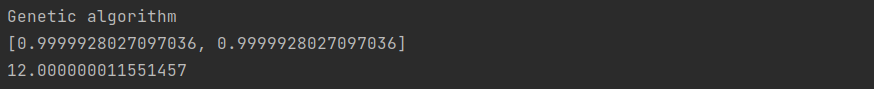
\includegraphics[width=0.8\textwidth]{img2}
\caption{Результаты работы генетического алгоритма}
\label{fig:img2}
\end{figure}

\section{Выводы}\label{Sect::conclusion}

В результате выполнения лабораторной работы были изучены алгоритмы многомерного поиска, генетический алгоритм, разработаны программы реализации алгоритмов многомерного поиска и генетического алгоритма.

\end{document}
